\documentclass[14pt,a4paper]{article}
\usepackage[T2A]{fontenc}
\usepackage[utf8]{inputenc}
\usepackage{amssymb}
\usepackage[russian]{babel}
\usepackage{amsmath}

%Картинки
\usepackage{graphicx}
%Папка с картинками
\graphicspath{{images/}}
%ИСпользуемые форматы
\DeclareGraphicsExtensions{.eps,.bmp,.jpg,.png}
\usepackage{caption}
%Подпись к картинкам
\captionsetup[figure]{name=Рисунок,labelsep=endash,font={Large}}
\usepackage{listings}

\usepackage{listings}
\usepackage{algorithm2e}

\usepackage{tocloft}
\usepackage{geometry}
%Настройка полей страницы
\geometry{left=3.0cm}
\geometry{right=1.0cm}
\geometry{top=2cm}
\geometry{bottom=2cm}

\newcommand{\biggI}{\renewcommand{\baselinestretch}{1.3}}
% команда \biggI для полуторного межстрочного интервала
\makeatletter
\renewcommand{\@oddfoot}{\hfil \Large \arabic{page}\hfil}
\renewcommand{\@evenfoot}{\hfil \Large \arabic{page}\hfil}
\makeatother
\renewcommand{\thepage}{\hfil \Large \arabic{page}\hfil}

\usepackage{indentfirst} % Красная строка

\fontencoding{T1}
\fontfamily{pcr}
\selectfont


\usepackage{pdfpages}

 %---------------- заголовки ----------- %
\usepackage{titlesec}
\usepackage{enumerate}
\titleformat{\chapter}[display]
    {\filcenter}
    {\MakeUppercase{\chaptertitlename} \thechapter}
    {8pt}
    {\bfseries}{}
 
\titleformat{\section}[block]
    {\Large\bfseries\sloppy\righthyphenmin62}
    {\thesection}
    {1em}{}
 
\titleformat{\subsection}[block]
    {\Large\bfseries\sloppy\righthyphenmin62}
    {\thesubsection}
    {1em}{}

\titleformat{\subsubsection}[block]
    {\Large\bfseries\sloppy\righthyphenmin62}
    {\thesubsubsection}
    {1em}{}


\usepackage{titletoc}
\titlecontents{section}
[2.6em] % ie, 1.5em (chapter) + 2.3em
{\sloppy\righthyphenmin62}
{\contentslabel{2.6em}}
{\hspace*{-2.6em}}
{\titlerule*[1pc]{}\contentspage}

\titlecontents{subsection}
[2.6em] % ie, 1.5em (chapter) + 2.3em
{\sloppy\righthyphenmin62}
{\contentslabel{2.6em}}
{\hspace*{-2.6em}}
{\titlerule*[1pc]{}\contentspage}

\titlecontents{subsubsection}
[2.6em] % ie, 1.5em (chapter) + 2.3em
{\sloppy\righthyphenmin62}
{\contentslabel{2.6em}}
{\hspace*{-2.6em}}
{\titlerule*[1pc]{}\contentspage}


    
% Настройка вертикальных и горизонтальных отступов
% Настройка вертикальных и горизонтальных отступов
\titlespacing{\section}{\parindent}{15mm}{10mm}
\titlespacing{\subsection}{\parindent}{15mm}{10mm}
\titlespacing{\subsubsection}{\parindent}{15mm}{10mm}

%------- конец заголовков --------- %


\lstdefinelanguage{cs}
  {morekeywords={abstract,event,new,struct,as,explicit,null,switch
		base,extern,object,this,bool,false,operator,throw,
		break,finally,out,true,byte,fixed,override,try,
		case,float,params,typeof,catch,for,private,uint,
		char,foreach,protected,ulong,checked,goto,public,unchecked,
		class,if,readonly,unsafe,const,implicit,ref,ushort,
		continue,in,return,using,decimal,int,sbyte,virtual,
		default,interface,sealed,volatile,delegate,internal,short,void,
		do,is,sizeof,while,double,lock,stackalloc,
		else,long,static,enum,namespace,string, },
	  sensitive=false,
	  morecomment=[l]{//},
	  morecomment=[s]{/*}{*/},
	  morestring=[b]",
}

\setlength\cftaftertoctitleskip{11mm}
\renewcommand{\cftdot}{}
  
\parindent=1.25cm % абзацный отступ
\biggI


\thispagestyle{empty} % не ставим номер страницы
\usepackage{float}%"Плавающие" картинки
\newcommand{\imgh}[3]{
\begin{figure}[H]
\center{
\includegraphics[width=#1]{#2}}
\caption{#3}
\label{ris:#2}
\end{figure}
}

\makeatletter
\renewcommand{\@biblabel}[1]{#1.}   % Заменяем библиографию с квадратных скобок на точку:
\makeatother

% новая команда \RNumb для вывода римских цифр
\newcommand{\RNumb}[1]{\uppercase\expandafter{\romannumeral #1\relax}}

%  маркированные списки
\renewcommand{\labelitemi}{-}
\renewcommand{\labelitemii}{-}
%  нумерованные списки
\renewcommand{\labelenumi}{\arabic{enumi})}
\usepackage{enumitem}
\setlist{nosep, leftmargin=\parindent}

%Начало документа
\begin{document}
\renewcommand*\contentsname{\parindent=1.25cm Содержание}
\Large
\setcounter{page}{2} % начать нумерацию с номера три

\newpage
% это оглавление, которое генерируется автоматически
\tableofcontents 
\Large
\setcounter{secnumdepth}{-1}

%Введение
\newpage
\section{Введение}
На протяжении всего времени существования человечества проблема возникновения, исследования и лечения различных заболеваний у человека является важной задачей медицинской деятельности. Особенно это касается онкологических заболеваний. На сегодняшний день нет четкой причины, по которой люди заболевают раком, но существует множество способов ранней диагностики таких заболеваний~\cite{fear2000}.
\par В данной работе рассматривается использование результатов моделирования, соответствующих методике микроволновой радиотермометрии молочных желез на основе работы специального диагностического комплекса РТМ-01-РЭС~\cite{problemiIzmereniyaVolsu}. Также рассматриваются популярные алгоритмы классификации данных и библиотеки для языка программирования Python, реализующие данные алгоритмы.
\par Главной целью работы является проведение исследования влияния размеров опухоли на точность  диагностики раковых заболеваний на основе данных микроволновой радиотермометрии, полученных в ходе компьютерного моделирования. Так как проведение классификации только на температурных данных может не дать хорошего результата, необходимо выявить какой из алгоритмов будет лучше работать с разными размерами опухоли и вариациями остальных параметров.


\setcounter{secnumdepth}{3}

%Глава 1
\newpage
\section{\Large Алгоритмы классификации данных}
Классификация данных состоит из прогнозирования определенного результата на основе уже известных данных. Чтобы предсказать результат, алгоритм обрабатывает данные, содержащие набор атрибутов и соответствующий каждому набору результат, обычно называемый атрибутом прогнозирования цели или классом~\cite{hetal2016}. Формируется модель алгоритма, которая пытается обнаружить отношения между атрибутами, которые позволили бы предсказать результат~\cite{kumbhar}. Такая процедура называется обучением модели, а набор данных, используемый для этого -- тестовой выборкой~\cite{Mirmozaffari}.
\par
Следующим шагом после обучения модели является прогнозирование -- процедура определения класса, при которой используется набор данных с неизвестными классами. Такой набор данных, который содержит тот же набор атрибутов, за исключением атрибута прогнозирования, часто называют тестовой выборкой~\cite{tprogeralgorithms}.
\par
Алгоритм анализирует входные данные и выдает прогноз. Точность прогноза определяет, насколько «хорош» алгоритм. Например, в медицинской базе данных обучающий набор должен иметь соответствующую информацию о пациенте, записанную ранее, где атрибутом прогноза является наличие или отсутствие у пациента проблем со здоровьем.
\par
Для определения того, какой именно алгоритм использовать для конкретной задачи можно воспользоваться схемой, изображенной на рисунке~\ref{ris:scikitlearn-map}. Исходя из того, что в текущей задаче используется не тестовая информация и имеется 160 примеров, то были выбраны алгоритмы SVM, k-ближайших соседей и наивный байесовский классификатор, описанные ниже.
\\
\imgh{1\linewidth}{scikitlearn-map}{Схема для определения алгоритма классификации для конкретной задачи}
\subsection{Метод опорных векторов}
Метод опорных вектором или SVM -- это метод статистической классификации~\cite{kristianini}. Он широко используется для задач различного рода и хорошо себя в них показывает~\cite{crammer}.
\par
Основной идеей метода является представление атрибутов данных в виде векторов и переход в пространство более высокой размерности, чем получившееся на этапе представления векторами. Затем ищется гиперплоскость с максимальным зазором в пространстве между объектами разных классов~\cite{rashka}~\cite{statnikov}.
\par
На рисунке~\ref{ris:svm_example} показан пример классификации методом SVM. Красной линией выделена как раз та самая гиперплоскость, четко разделяющая объекты разных классов друг от друга.
\\
\imgh{1\linewidth}{svm_example}{Пример классификации методом SVM}
\par
Алгоритм может использоваться с одним из следующих видов ядер~\cite{crammer}:
\begin{itemize}
	\item[-] Полиномиальное (однородное) $k(x,x^{'}) = (x \cdot x^{'})^{d}$;
	\item[-] Полиномиальное (неоднородное) $k(x,x^{'}) = (x \cdot x^{'} + 1)^{d}$;
	\item[-] Радиальная базисная функция $k(x,x^{'}) = exp(-\gamma ||x - x^{'}||^{2})$, для $\gamma > 0$;
	\item[-] Радиальная базисная функция Гаусса $k(x,x^{'}) = exp\left ( -\frac{||x - x^{'}||^{2}}{2\sigma^{2}} \right )$;
	\item[-] Сигмоид $k(x,x^{'}) = tanh(kx\cdot x^{'} + c)$.
\end{itemize}
\subsection{Метод k-ближайших соседей}
Алгоритм k-ближайших соседей является простым статистическим алгоритмом обучения, в котором объект классифицируется своими соседями. При классификации таким методом объект относится к классу, наиболее распространенному среди его k-ближайших соседей~\cite{potapov}~\cite{flah}. Пример классификации приведен на рисунке~\ref{ris:knn_example}, где в качестве классифицируемого объекта используется прямоугольник и существует несколько объектов известных классов -- белые точки и черные. Замерив расстояние от объекта до его соседей с различными классами и основываясь на методе k-ближайших соседей данный объект будет отнесен к классу черный точек, а не белых.
\\
\imgh{1\linewidth}{knn_example}{Пример классификации методом k-ближайших соседей}
\par
При нахождении атрибутов учитывается значимость атрибутов и часто применяется прием растяжения осей, демонстрируемый в формуле~\eqref{eq:eq1}. Использование данного приема снижает ошибку классификации.
\begin{equation}\label{eq:eq1}
D_{E} = \sqrt{3(x_{A} - y_{A})^{2} + (x_{B} - y_{B})^{2}},
\end{equation}
где $x_{A}, y_{A}$ -- значения атрибута A в наборе данных, $x_{B}, y_{B}$ -- значения атрибута B.
\par
Данный алгоритм возможно применять как для данных с маленьким количеством атрибутов, так и с достаточно большим. Важным моментом при работе с алгоритом является определение функции расстояния между значениями. Примером такой функции может быть евклидово расстояние -- формула~\eqref{eq:eq2}.
\begin{equation}\label{eq:eq2}
D_{E} = \sqrt{\sum_{i}^{n}(x_{i} - y_{i})^{2}},
\end{equation}
где $x_{i}, y_{i}$ -- значения атрибутов в наборе данных.
\subsection{Наивный байесовский классификатор}
Наивный байесовский классификатор является простым вероятностным классификатором и основывается на применении теоремы Байеса со строгими предположениями о независимости~\cite{potapov}~\cite{danilovsv}. Хотя наивный байесовский классификатор редко применим к большинству реальных задач, но зачастую в определенных задачах он демонстрирует хорошие результаты и часто конкурирует с более сложными методами, такими как SVM и классификационным деревьями~\cite{Mirmozaffari}. Классификация данным методом очень зависит от распределения зависимостей атрибутов, а не от самих зависимостей~\cite{juravlev}.
\par
Вероятностная модель классификатора:
\begin{equation}\label{eq:eq3}
p(C|F_{1},...,F_{n}) = \frac{p(C)p(F_{1},...,F_{n}|C)}{p(F_{1},...,F_{n})},
\end{equation}
где $C$ -- класс модели, а $F_{i}$ -- классифицируемые модели~\cite{Mirmozaffari}.
\par
Использование формулы~\eqref{eq:eq3} при классификации дает минимально значение среднего риска или математичского ожидания ошибки:
\begin{equation}\label{eq:eq4}
R(a) = \sum_{y\in Y}\sum_{\varsigma\in Y}\lambda_{y}P_{y}P_{x,y}\left\lbrace a(x)=\varsigma|y \right\rbrace ,
\end{equation}
где $\lambda_{y}$ -- цена ошибки при отнесении объекта класса $Y$ к какому-либо другому классу.
%------------------------------------------------------------------------------------------------------
%------------------------------------------------------------------------------------------------------


%Глава 2
\newpage
\section{\Large Глава}
Текст.
\subsection{Подглава}
Текст

%------------------------------------------------------------------------------------------------------
%------------------------------------------------------------------------------------------------------


%Глава 3
\newpage
\section{\Large Классификация температурных данных компьютерного моделирования}\vspace{-7mm}
\subsection{Данные для классификации}
В работе использовались данные компьютерного моделирования яркостной температуры молочных желез больных и здоровых пациентов. Данные были представлены в виде девяти значений температуры на поверхности кожи и девяти значений внутренней температуры, согласно методике обследования методом радиотермометрии. Схема расположения точек при замере температур представлена на рисунке~\ref{ris:rtm-res-scheme}. Отдельным атрибутом являлся класс модели. Для здоровых моделей значения класса было равно нулю, а для больных -- единице. Исходя из количества классов, классификацию в данной работе можно считать бинарной.
\\
\imgh{0.75\linewidth}{rtm-res-scheme}{Пример данных температурных данных компьютерного моделирования, где в столбце «target» здоровые — «0», больные — «1»}
\par
Для исследования были взяты температурные данные моделей с радиусом опухоли 0.5 см и 0.75 см. Данные были представлены в виде двух CSV-файлов, в которых находилось по 160 моделей для каждого размера опухоли соответственно (рисунок~\ref{ris:data_example}). Одна половина моделей состояла из здоровых пациентов, а другая из больных. На подготовительном этапе данные были разбиты на обучающую и тестовую выборки в соотношении один к четырем.
\\
\imgh{1\linewidth}{data_example}{Пример данных температурных данных компьютерного моделирования, где в столбце «target» здоровые — «0», больные — «1»}

%------------------------------------------------------------------------------------------------------

\subsection{Частотный анализ классифицируемых данных}
Перед классификацией температурных данных был проведен частотный анализ для исследования распределения температуры в зависимости от того, в какой точке она была замерена и есть ли у данной модели опухоль. Частотный анализ был произведен с помощью библиотеки Pandas, а графическое отображение результатов с помощью Matplotlib. Точки, которые были проанализрованы соответствуют точкам на схеме измерений согласно методу РТМ (рисунок~\ref{ris:rtm-res-scheme}). 
\par
Сначала для исследования была взяла точка 0ртм. Результаты исследования представлены в виде диаграммы частот (рисунок~\ref{ris:0rtm}), где верхняя диаграмма -- это здоровые пациенты, а нижняя -- больные.
\imgh{1\linewidth}{0rtm}{Диаграмма частот температур в точке 0ртм. Верхняя диаграмма — здоровые пациенты, нижняя — больные}
\par
Изучив диаграммы, можно заметить, что в данной точке у пациентов чаще встречаются более высокие температуры, нежели у здоровых. Точка 0ртм больше всего подверждена воздействию от опухоли в температурном смысле, так как находится ровно в центре молочной железы.
\par
Следующей для исследования была рассмотрена точка 3ртм, диаграмма частот температур которой представлена на рисунке~\ref{ris:3rtm}. Для данной точки можно наблюдать схожую картину с точкой 0ртм -- тут так же больше значений со средней температурой у больных пациентов, несмотря на то, что эта точка не является центральной.
\imgh{1\linewidth}{3rtm}{Диаграмма частот температур в точке 3ртм. Верхняя диаграмма — здоровые пациенты, нижняя — больные}
\par
Также была рассмотрена точка 7ртм, для которой как видно из диаграммы частот температур (рисунок~\ref{ris:7rtm}) ситуация аналогична с точками 0ртм и 3ртм.
\imgh{1\linewidth}{7rtm}{Диаграмма частот температур в точке 7ртм. Верхняя диаграмма — здоровые пациенты, нижняя — больные}

%------------------------------------------------------------------------------------------------------

\subsection{Результаты классификации для моделей с опухолью радиусом 0.5 см}
Для моделей с разными размерами опухоли отдельно была посчитана точность определения класса и построены круговые диаграммы для наглядности, где как «1» отмечены верно классифицированные модели, а как «0» -- неверно классифицированные.
\par
Как видно из диаграммы на рисунке~\ref{ris:05}, для моделей с радиусом опухоли 0.5 см лучший результат показал метод SVM, точность определения классов которого равна 57.5\%. Хуже всего для данных моделей показал себя наивный байесовский классификатор с точностью классификации 27.5\%
\imgh{1\linewidth}{05}{Диаграммы с точностью определения класса для трех методов классификации моделей с размером опухоли R=0.5 см («1» – классифицировано верно, «0» – классифицировано неверно)}

%------------------------------------------------------------------------------------------------------
\subsection{Результаты классификации для моделей с опухолью радиусом 0.75 см}
Рассмотрим результаты классификации для моделей с радиусом опухоли 0.75 см (рисунок~\ref{ris:075}). Как видно из диаграмм, для данных моделей наивный байесовский классификатор сработал лучше, для для моделей с радиусом опухоли 0.5 см, показав результат точности равный 70\%. Точность определения классов методом SVM опять оказалась лучше, чем у остальных -- 72.5%.
\par
Исходя из этого, можно сделать вывод, что точность классификации сильно зависит от размеров опухоли и выбранного алгоритма классификации.
\imgh{1\linewidth}{075}{Диаграммы с точностью определения класса для трех методов классификации моделей с размером опухоли R=0.75 см («1» – классифицировано верно, «0» – классифицировано неверно)}

%------------------------------------------------------------------------------------------------------

\subsection{Результаты классификации для всех моделей вместе}
В качестве заключительного эксперимента было принято решение смешать вместе данные моделей с радиусом 0.5 см и 0.75 см. В качестве обучающей выборки использовались 180 моделей, а в качестве тестовой -- 60 моделей. После чтения из файла данные были перемешаны между собой. 
\par
Результаты представлены на диаграмме (рисунок~\ref{ris:075}). В этот раз лучшим по точности определения класса стал наивный байесовский классификатор с точностью 70\%, которая не изменилась по сравнению с предыдущим экспериментом. А метод  SVM, показавший лучший результат в предыдущих двух экспериментах, в этот раз определил классы моделей с точностью 66.7\%, такой же как и метод k-ближайших соседей.
\imgh{1\linewidth}{all}{Диаграммы с точностью определения класса для трех методов классификации моделей с размером опухоли R=0.5 см и R=0.75 см вместе («1» – классифицировано верно, «0» – классифицировано неверно)}

%------------------------------------------------------------------------------------------------------
%------------------------------------------------------------------------------------------------------


\setcounter{secnumdepth}{-1}

%Заключение
\newpage
\section{Заключение}
В данной работе были рассмотрены некоторые из популярных библиотек языка программирования Python для решения задач машинного обучения. Был описан принцип работы таких алгоритмов классификации как метод опорных векторов (SVM), k-ближайших соседей и наивный байесовский классификатор.
\par
Реализована программа для классификации данных компьютерного моделирования яркостной температуры на языке Python с помощью библиотеки Scikit-learn. Температурные данные были разбиты на обучающую и тестовую выборки и классифицированы с помощью получившейся программы.
\par
Исходя из результатов классификации моделей был сделан вывод, что точность классификации данных сильно зависит от используемого алгоритма и размеров опухоли. Причем, если использовать все данные вместе -- то результат сильно отличается от экспериментов, проведенных для каждого размера опухоли отдельно. Лучше всего в проведенных экспериментах себя показал метод опорных векторов (SVM) и наивный байесовский классификатор.

%Список литературы
\newpage
\addcontentsline{toc}{subsection}{Список литературы}
\begin{thebibliography}{3}
	\bibitem{bardati} Bardati, F. Modeling the Visibility of Breast Malignancy by a MicrowaveRadiometer / F. Bardati, S. Iudicello. -- Текст : непосредственный // Biomed. Engineering. -- 2008. -- Vol.55 (6). -- С. 214-221.
	
	\bibitem{kristianini} Cristianini, Т. An Introduction to Support Vector Machines and Other Kernel-based Learning Methods / Nello Cristianini, John Shawe-Taylor. -- Текст : непосредственный // Cambridge University Press. -- 2000. -- 204 с.
	
	\bibitem{crammer} Crammer, K. On the algorithmic implementation of multiclass kernel-based vector machines / Koby Crammer, Yoram Singe. -- Текст : непосредственный // Journal of Machine Learning Research. -- 2002. -- № 2. -- С. 265–292.
	
	\bibitem{fear2000} Fear, K.E. Microwave detection of breast cancer / K.E. Fear, M. Ctuchly. -- Текст : непосредственный // IEEE Trans. Microwave Theory Tech. -- 2000. -- Vol.48 (11). -- С. 1854-1863.
	
	\bibitem{hetal2016} Hetal, B. An Empirical Evaluation of Data MiningClassification Algorithms / He-tal Bhavsar, Amit Ganatra. — Текст : непосредственный // International Journal of Computer Scienceand Information Security (IJCSIS). — 2016 — № 5. — С. 142–150. 
	
	\bibitem{kumbhar} Kumbhar, S. Comparative Analysis of Classification Algorithms / Vijaykumar S. Kumbhar. -- Текст : электронный // NCORTIT. -- 2017. -- 5 С. -- URL: https://www.researchgate.net/publication/313440536, свободный. — Загл. с экрана.
	
	\bibitem{leroy1998} Leroy, Y. Non-invasive microwave radiometry thermometry / Y. Leroy, B. Bocquet, A. Mammouni. -- Текст : непосредственный // Physiol. Means. -- 1998. -- Vol.19. -- С. 127-148.
	
	\bibitem{Mirmozaffari} Mirmozaffari, M. Data Mining Classification Algorithms for Heart Disease Prediction / Mirpouya Mirmozaffari, Alireza Alinezhad, Azadeh Gilanpour. -- Текст : непосредственный // n-ternational Journal of Computing Communications \& InstrumentationEngg (IJCCIE). -- 2017. -- 4, № 1 -- С. 11-15.
	
	\bibitem{mossina} Mossina, L. Naive Bayes Classification for Subset Selection / Luca Mossina, Emmanuel Rachelson. -- Текст : электронный // Physiol. Means. -- 1998. -- Vol.19. -- С. 127-148. -- URL: https://www.researchgate.net/publication/318560282, свободный. — Загл. с экрана.
	
	\bibitem{Sherwood2012} Sherwood, L. Fundamentals of Human Physiolog / L. Sherwood. -- Текст : непосредственный // Belmon : Brooks/Cole -- 2012. -- 720 с.
	
	\bibitem{statnikov} Statnikov, A. A Gentle Introduction to Support Vector Machines in Biomedicine: Theory and methods / Alexander Statnikov, Constantin F. Aliferis, Douglas P. Hardin. -- Текст : непосредственный // World Scientific. -- 2011. -- 183 с.
	
	\bibitem{stauffer2014} Stauffer, P.R. Utility of Microwave Radiometry for Diagnostic and Therapeutic Applications of Non-Invasive Temperature Monitoring / P.R. Stauffer, D.R. Rodrigues. -- Текст : непосредственный // IEEE BenMAS (Benjamin Franklin Symposium on Microwave and Antenna Sub-systems). -- 2014. -- С. 1-3.
	
	\bibitem{vanOngeval} Van Ongeval, Ch. Digital mammography for screening and diagnosis of breast cancer:
	an overview / Ch. Van Ongeval. -- Текст : непосредственный // PubMed PMID. -- 2007. -- Vol. 90 (3). -- С. 163–166.
	
	\bibitem{aivazyan} Айвазян , C. Прикладная статистика: классификация и снижение размерности / Айвазян С. А., Бухштабер В. М., Енюков И. С., Мешалкин Л. Д. -- Текст : непосредственный // Москва : Финансы и статистика, 1989. -- 487 с.
	
	\bibitem{tprogeralgorithms} Алгоритмы интеллектуального анализа данных. / Текст : электронный // 2015. -- URL: https://tproger.ru/translations/top-10-data-mining-algorithms/, свободный. — Загл. с экрана.
	
	\bibitem{barsegyan} Барсегян, А. Методы и модели анализа данных: OLAP и Data Mining / А.А. Барсегян, М.С. Куприянов, В.В. Степаненко, И.И. Холод. -- Текст : непосредственный // Санкт-Петербург : 
	БХВ-Петербург, 2004. -- 336 с.
	
	\bibitem{biryulinCOmsol} Бирюлин, Г. Теплофизический расчет в конечно-элементном пакете COMSOL/FEMLAB :  методическое пособие / Г.В. Бирюлин. -- Текст : непосредственный // Санкт-Петербург : СПбГУИТМО, 2006. -- 75 с.
	
	\bibitem{vanderplus} Вандер Плас, Д. Python для сложных задач. Наука о данных и машинное обучение / Дж. Вандер Плас. -- Текст : непосредственный // Санкт-Петербург : Питер, 2017. -- 576 с.
	
	\bibitem{vesninSovMicrowave} Веснин, С. Современная микроволновая радиотермометрия молочных желез / С.Г. Веснин, М.А. Каплан, Р.С. Авакян. -- Текст : электронный // Маммология/Онкогинекология. -- 2008. -- №3 -- 8 с. -- URL: https://elibrary.ru/item.asp?id=11610722, свободный. — Загл. с экрана.
	
	\bibitem{vesninDevSerii} Веснин, С. Разработка серии антенн-аппликаторов для неинвазивного измерения температуры тканей организма человека при различных патологиях / С.Г. Веснин, М.К. Седанкин. -- Текст : электронный // Вестник МГТУ им. Н.Э. Баумана. Сер. «Естественные науки». -- 2012. -- №11 -- С. 43-61. -- URL: https://elibrary.ru/item.asp?id=20179995, свободный. — Загл. с экрана.
	
	\bibitem{vyugin} Вьюгин, В. Математические основы теории машинного обучения и прогнозирования / Владимир Вьюгин. -- Текст : электронный // МЦМНО. -- 2013. -- 390 с.
	
	\bibitem{gudfellow} Гудфеллоу, Я.  Глубокое обучение / Гудфеллоу Я., Бенджио И., Курвилль А. -- Текст : электронный // Москва : ДМК Пресс. -- 2017. -- 652 с.	
	
	\bibitem{danilovsv} Данилов, С.  Интеллектуальный анализ данных с использованием системы Rapid
	Miner / С.В. Данилов. -- Текст : электронный // Казанский (Приволжский) федеральный университет. -- 2014. -- 43 с.			
	
	\bibitem{dauni} Дауни, А. Байесовские модели / Дауни А.Б., пер. с анг. В. А. Яроцкого -- Текст : непосредственный // Москва : ДМК Пресс. -- 2018. -- 182 с.				
	
	\bibitem{douson} Доусон, М. Программируем на Python / Доусон М. -- Текст : непосредственный // Санкт-Петербург : Питер. -- 2019. -- 416 с.	
	
	\bibitem{juravlev} Журавлев, Ю. «Распознавание». Математические методы. Программная система. Практические применения / Журавлев Ю. И., Рязанов В. В., Сенько О. В. -- Текст : непосредственный // Москва : Фазис, 2006. -- 176 с.
	
	\bibitem{levitin} Левитин, А. Алгоритмы. Введение в разработку и анализ / Левитин А. В. -- Текст : непосредственный // Москва : Вильямс. -- 2006. -- 576 с.		
	
	\bibitem{problemiIzmereniyaVolsu} Лосев, А. Проблемы измерения и моделирования тепловых и радиационных полей в биотканях: анализ данных микроволновой термометрии / А.Г. Лосев, А.В. Хоперсков, А.С. Астахов, Х.М. Сулейманова. -- Текст : непосредственный // Вестн. Волгогр. гос. ун-та. Сер. 1, Мат. Физ. -- 2015. -- No 6 -- 41 с.						
	
	\bibitem{makgrat} МакГрат, М. Алгоритмы. Python. Программирование для начинающих / Майк МакГрат. -- Текст : непосредственный // Эксмо. -- 2013. -- 194 с.							
	
	\bibitem{muller} Мюллер, А. Введение в машинное обучение с помощью Python. Руководство для специалистов по работе с данными / Андреас Мюллер, Сара Гвидо. -- Текст : непосредственный // Вильямс. -- 2017. -- 480 с.				
	
	\bibitem{nikolenko} Николенко, С. Алгоритмы. Глубокое обучение / Николенко С., Кадурин А., Архангельская Е. -- Текст : непосредственный // Санкт-Петербург : Питер. -- 2018. -- 480 с.
	
	\bibitem{paklin} Паклин, Н. Бизнес-аналитика: от данных к знаниям : Учебное пособие / Паклин Н.Б., Орешков В.И. -- Текст : непосредственный // Санкт-Петербург : Питер, 2013. -- 2-е изд. -- 704 с.
	
	\bibitem{potapov} Потапов, М. Анализ эффективности алгоритмов интеллектуального анализа данных для решения задачи распознавания изображений со спутников / Потапов М. П. -- Текст : электронный // Федеральное государственное бюджетное образовательное учреждение высшего образования "Сибирский государственный университет науки и технологий имени академика М.Ф. Решетнева" : Актуальные проблемы авиации и космонавтики, 2016. -- 1. -- № 12 -- С. 563-565.	
	
	\bibitem{rashka} Рашка, С. Python и машинное обучение / Рашка С., пер. с англ. А. В. Логунова. -- Текст : непосредственный // Москва : ДМК Пресс, 2017. -- 418 с.		
	
	\bibitem{rozenblatt} Розенблатт, Ф. Принципы нейродинамики: Перцептроны и теория механизмов мозга / Розенблатт Ф. -- Текст : непосредственный // Москва : Мир, 1965. -- 480 с.	
	
	\bibitem{flah} Флах, П. Машинное обучение / Флах П. -- Текст : непосредственный // Москва : ДМК Пресс, 2015. -- 400 с.
	
	\bibitem{shlezinger} Шлезингер, М. Десять лекций по статистическому и структурному распознаванию / Шлезингер М., Главач В. -- Текст : непосредственный // Киев : Наукова думка, 2004. -- 546 с.
	
\end{thebibliography}

%Приложения
\newpage
\addcontentsline{toc}{section}{Приложение А} 
\begin{center} 
    \textbf{Приложение А}
\end{center} 
\vspace{8mm}
\par
Листинг А.1 -- Подпись
\vspace{8mm}
\large
\begin{verbatim}
class HelloWorld
{
    MessageBox.Show("Hello world!");         
}
\end{verbatim}
\vspace{8mm}
\Large

%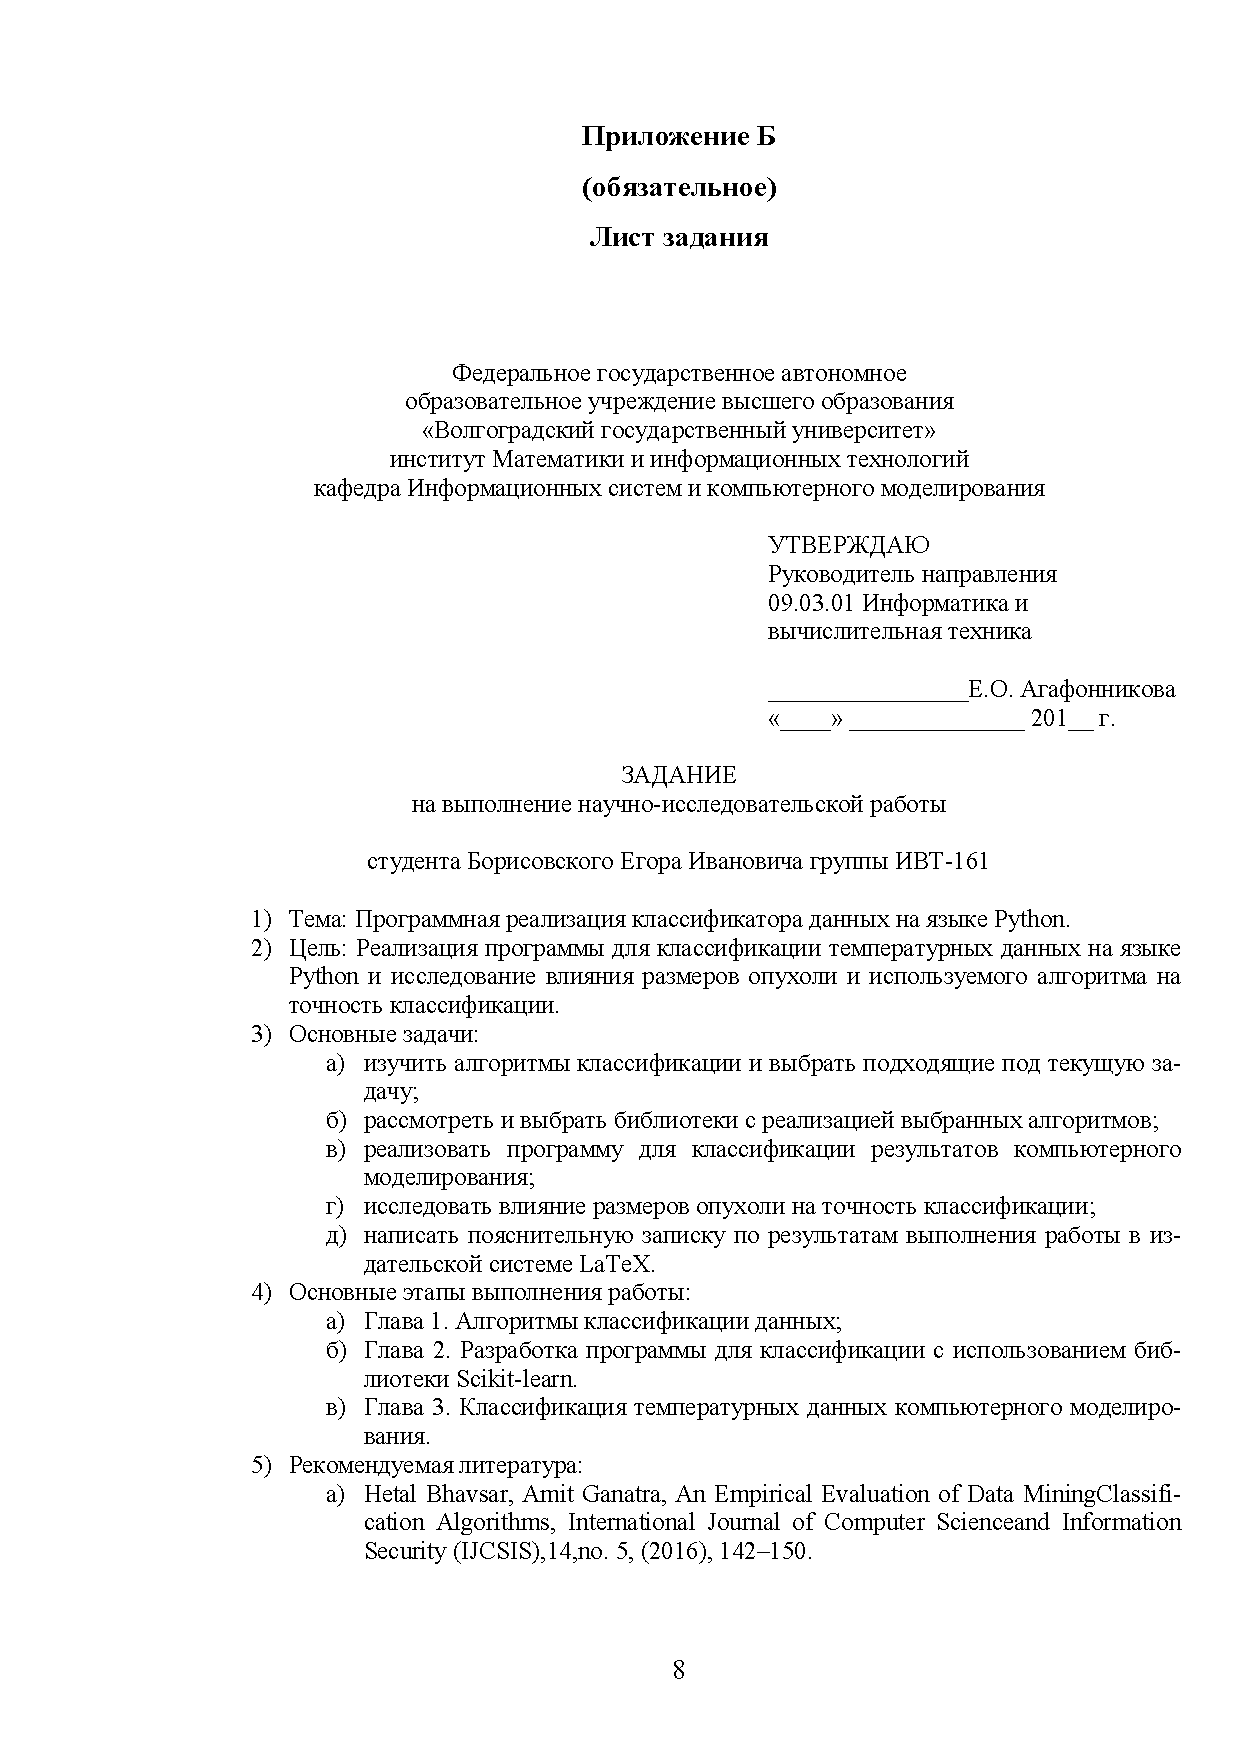
\includepdf[pages=-]{tz.pdf}

\end{document}